\documentclass[11pt,letterpaper]{article}
\usepackage[utf8]{inputenc}
\usepackage[T1]{fontenc}
\usepackage{amsmath}
\usepackage{amsfonts}
\usepackage{amssymb}
\usepackage{graphicx}
\usepackage{IEEEtrantools}
\usepackage{float}
\usepackage[newfloat]{minted}
\usepackage{caption}
\usepackage{tcolorbox}
\usepackage{etoolbox}
\newenvironment{code}{\captionsetup{type=listing}}{}
\SetupFloatingEnvironment{listing}{name=Code Block}
\BeforeBeginEnvironment{minted}{\begin{tcolorbox}}%
\AfterEndEnvironment{minted}{\end{tcolorbox}}%
\author{Alan Freeman}
\title{GAN Gogh: Use of a GAN to Imitate the Style of Vincent Van Gogh}
\begin{document}
	\setminted{breaklines, autogobble, tabsize=4, fontsize=\small}
% TODO: citations go inside periods.  I think.  Look it up.
% data.gov uses dataset as a single word, so we will adhere to that for this document
% TODO: You are not submitting this for publication, therefore you can afford to be frank with your null results
% eg talk about what you did that didn't work/ was a huge dumpster fire/ a giant waste of time, but WHY that is interesting knowledge.
% see replication crisis
	\maketitle
	\section{Introduction}
		\subsection{Background}
			A GAN (Generative Adversarial Network) is a type of artificial intelligence composed of two neural networks, first introduced by Goodfellow et al in 2014 \cite{NIPS2014_5ca3e9b1}.
			It takes its name from the fact that it uses two networks in direct opposition to each other.
			One, referred to as the generator, tries to generate images that resemble the training data.
			The other, called the discriminator, attempts to determine whether any given image is from the original dataset.

			%why does it get better at detecting fakes and how does generator improve
			% you can expand here.  More detail is better.
			As the discriminator gets better at detecting fakes, the generator has to improve the quality of its images in order to go undetected.
			This feedback loop produces images that become progressively more similar to the original input.
			The specific architecture of GAN that we used in this research was a Deep Convolutional GAN, or DCGAN, introduced by Radford et al in 2015\cite{radford2015unsupervised}.
		\subsection{Motivation}
			By training our GAN on images of paintings by Vincent Van Gogh, we hope to learn what specific features make his artwork so immediately recognizable.
			Towards this purpose, we collected 211 images from the Van Gogh Museum's website for use in training.
			Furthermore, we hope to create a tool that others can use to easily train their own GANs on their own data.

	\section{How We Approached Our Goal}
		To accomplish our goals, we assembled a Jupyter notebook that trains a DCGAN on user-specified data.
		Large parts of our code come from the TorchGAN\cite{pal2019torchgan} project's tutorial examples.
		\begin{code}
			\caption{}
			\begin{minted}{python3}
				try:
					import torchgan
					print(f"Existing TorchGAN {torchgan.__version__} installation found")
				except ImportError:
					import subprocess
					import sys
					subprocess.check_call([sys.executable, "-m", "pip", "install", "torchgan"])
					import torchgan
					print(f"Installed TorchGAN {torchgan.__version__}")
			\end{minted}
			\label{code:block1}
		\end{code}
		Code block \ref{code:block1} checks whether the environment in which the notebook is running has TorchGAN installed, and installs it if missing.
		This block is primarily included for interoperability with Google Colab, which does not have TorchGAN installed by default.
		\begin{code}
			\caption{}
			\begin{minted}{python3}
				import torch
				import torch.nn as nn
				import torch.backends.cudnn
				import torch.utils.data as tdata
				from torch.optim import Adam
				import torchvision
				import torchvision.datasets as dsets
				from torchvision.datasets import ImageFolder
				import torchvision.transforms as transforms

				import numpy as np
				import matplotlib.pyplot as plt

				import torchgan
				from torchgan.models import *
				from torchgan.losses import *
				from torchgan.trainer import Trainer
			\end{minted}
			\label{code:block2}
		\end{code}
		Code block \ref{code:block2} contains all of the import statements required for the rest of the code.
		\begin{code}
			\caption{}
			\begin{minted}{python3}
				size = 128
				grayscale = False
				folder = "./relative/path/to/images/"

				if grayscale:
					channels = 1
					data = ImageFolder(
						root=folder,
						transform=transforms.Compose([
							transforms.Resize((size, size)),
							transforms.ToTensor(),
							transforms.Grayscale(),
							transforms.Normalize(mean=.5, std=.5)
						])
					)
				else:
					channels = 3
					data = ImageFolder(
						root=folder,
						transform=transforms.Compose([
							transforms.Resize((size, size)),
							transforms.ToTensor(),
							transforms.Normalize(mean=.5, std=.5)
						])
					)
				print(len(data))
			\end{minted}
			\label{code:block3}
		\end{code}
		Code block \ref{code:block3} uses a class from the TorchVision package of Torch to set up the dataset that the GAN will be training on.
		Figuring out how to write the code for this block was quite time-consuming, and included multiple false starts.
		Our first attempt involved reading the files and converting them to NumPy arrays, then saving each array to a file.
		However, we then realized that this solution wasn't actually compatible with the TorchGAN code, so we started going through the documentation of the built-in datasets to figure out what we should subclass.
		Once we found the appropriate class, we began writing a custom dataset class that would allow the user to specify a directory, and from that, load all of the images in that directory as a dataset.
		We then learned that this was almost exactly the same usage and behavior as the already-existing ImageFolder class in the TorchVision package, so we switched to using that instead.
		A large amount of effort was spent performing a deep dive into novel and unfamiliar tools; doing so allowed us to become more familiar with the internal structure of the package, which increased our understanding of how the code works.

		Functionally, the block creates an ImageFolder object in memory from the directory provided.
		The images are scaled to the specified size, normalized, and, if specified, converted to grayscale.

		Code blocks \ref{code:block4}, \ref{code:block5}, \ref{code:block6}, \ref{code:block7}, and \ref{code:block9} are all adapted from the TorchGAN tutorial.
		\begin{code}
			\caption{}
			\begin{minted}{python3}
				dataloader = tdata.DataLoader(data, batch_size=64, shuffle=True)
			\end{minted}
			\label{code:block4}
		\end{code}
		Code block \ref{code:block4} loads the object created in code block \ref{code:block3} into Torch's DataLoader class, which will be passed to the final Trainer object in either code block \ref{code:block9} or \ref{code:block10}, depending on use case.
		\begin{code}
			\caption{}
			\begin{minted}{python3}
				dcgan_network = {
					"generator": {
						"name": DCGANGenerator,
						"args": {
							"encoding_dims": 100,
							"out_size": size,
							"out_channels": channels,
							"step_channels": 32,
							"nonlinearity": nn.LeakyReLU(0.2),
							"last_nonlinearity": nn.Tanh(),
						},
						"optimizer": {"name": Adam, "args": {"lr": 0.0001, "betas": (0.5, 0.999)}},
					},
					"discriminator": {
						"name": DCGANDiscriminator,
						"args": {
							"in_size": size,
							"in_channels": channels,
							"step_channels": 32,
							"nonlinearity": nn.LeakyReLU(0.2),
							"last_nonlinearity": nn.LeakyReLU(0.2),
						},
						"optimizer": {"name": Adam, "args": {"lr": 0.0003, "betas": (0.5, 0.999)}},
					},
				}
			\end{minted}
			\label{code:block5}
		\end{code}
		Code block \ref{code:block5} constructs the objects that make up the DCGAN itself.
		Values from code block \ref{code:block3} are used to configure the generator and discriminator objects so that they are compatible with the input images.
		\begin{code}
			\caption{}
			\begin{minted}{python3}
				minimax_losses = [MinimaxGeneratorLoss(), MinimaxDiscriminatorLoss()]
				wgangp_losses = [
				WassersteinGeneratorLoss(),
				WassersteinDiscriminatorLoss(),
				WassersteinGradientPenalty(),
				]
				lsgan_losses = [LeastSquaresGeneratorLoss(), LeastSquaresDiscriminatorLoss()]
			\end{minted}
			\label{code:block6}
		\end{code}
		Code block \ref{code:block6} sets up three potential objects for measuring the GAN's progress.
		Only one is needed for any given model, but having multiple available allows the user to easily experiment with different configurations.
		Due to time constraints, all of our training was done using the same set of losses.
		\begin{code}
			\caption{}
			\begin{minted}{python3}
				if torch.cuda.is_available():
				device = torch.device("cuda:0")
				# Use deterministic cudnn algorithms
				torch.backends.cudnn.deterministic = True
				epochs = 10
				else:
				device = torch.device("cpu")
				epochs = 5

				print("Device: {}".format(device))
				print("Epochs: {}".format(epochs))
			\end{minted}
			\label{code:block7}
		\end{code}
		Code block \ref{code:block7} detects what hardware is available for use in training.
		It also sets a default value for number of epochs based on the available hardware.
		If a device that uses NVIDIA's CUDA technology is available, that device is preferred.
		Otherwise, the CPU is used.
		\begin{code}
			\caption{}
			\begin{minted}{python3}
				epochs = 700

				trainer = Trainer(
				dcgan_network,
				lsgan_losses,
				sample_size=64,
				epochs=epochs,
				device=device
				)
			\end{minted}
			\label{code:block8}
		\end{code}
		Code block \ref{code:block8} constructs the Trainer object that trains the model.
		This block will have to be re-run with a new epochs value each time the user wishes to continue training an existing model.
		\begin{code}
			\caption{}
			\begin{minted}{python3}
				trainer(dataloader)
			\end{minted}
			\label{code:block9}
		\end{code}
		Code block \ref{code:block9} performs the training from the beginning.
		\begin{code}
			\caption{}
			\begin{minted}{python3}
				model = "./model/gan4.model"

				trainer.load_model(model)
				trainer(dataloader)
			\end{minted}
			\label{code:block10}
		\end{code}
		Code block \ref{code:block10} loads in a previously-created model and then resumes training on it.
		Due to the way that TorchGAN works, a new Trainer object is required to resume training, as each Trainer has a set number of epochs that it will train until.
		If, for example, you were to load a model that had already been trained for 100 epochs into a Trainer set to train for 100 epochs, the Trainer would not perform any additional training, as the target number has already been reached.
	\section{How to Use Our Code}
		If you are running our code on Colab, be sure to either run code block \ref{code:block1} or manually install TorchGAN, as Colab doesn't have it installed by default.

		Code block \ref{code:block2} can be run as-is.

		Code block \ref{code:block3} requires some configuration before being run.
		First, choose the size of the images.
		This number must be an exact power of 2, and no smaller than 16.
		Larger values have the potential to create more detailed images, but will increase the time it takes to train.
		Second, if the images you are using are in black and white, set the grayscale variable to "True".
		Finally, specify the folder that the images are in.
		Due to the way that Torch's code works, you will have to specify the folder that contains the folder you want.
		This may require making a new folder and moving your folder into it.

		Code blocks \ref{code:block4}, \ref{code:block5}, \ref{code:block6}, and \ref{code:block7} can be run as-is.

		Before running code block \ref{code:block8}, you may choose to override the number of epochs that the model will train for.
		More epochs will take longer, but allow the model to become more refined.
		You can always resume training from a saved model later on.

		Code block \ref{code:block9} should only be used if you are creating a brand new model.
		To resume training a previous model, use code block \ref{code:block10}.

		Code block \ref{code:block10} is used to continue training.
		In the first line of the block, specify the path to an existing model.
		The default value is the location that the notebook uses to save checkpoints.
		It should always be the most recent model, as long as the number of epochs was divisible by five.
		If you are running the notebook on Colab, you will need to manually save and upload your .model files, as Colab clears user data between sessions.

	\section{Generation of Results}
		\subsection{Parameters Used}
			The primary parameter which we manipulated was the training dataset.
			The datasets that we used were as follows:
			\begin{enumerate}
				\item The MNIST dataset (60,000 images)
				\item The images that we collected from the Van Gogh Museum (211 images)
				\item The Van Gogh images collected by the CycleGAN researchers (400 images)
				\item The Monet images collected by the CycleGAN researchers (1,000 images)
				\item The Monet images collected by the CycleGAN researchers, converted to grayscale (1,000 images)
				\item The landscape images collected by Jones and Bonafilia\cite{otherGanGogh} (15,000 images)
			\end{enumerate}
			Another parameter was the resolution of the images.
			The order of the values in the following list correspond to the order of the datasets listed above.
			\begin{enumerate}
				\item 32 by 32 pixels
				\item 256 by 256 pixels
				\item 256 by 256 pixels
				\item 256 by 256 pixels
				\item 256 by 256 pixels
				\item both 64 by 64 pixels and 128 by 128 pixels  % mention that 128x128 was not feasible given time/equipment constraints and would most likely be reasonable if either restraint was removing
			\end{enumerate}
			All other parameters remained constant between models.
		\subsection{Results}
		%TODO: if possible expand on captions
			\subsubsection{Model 1: Van Gogh Museum Dataset}
				This model was our first attempt at our goal.
				For the first thousand or so epochs of training, the model produced nothing but static, with occasional blue patches.\footnote{Each figure is composed of a grid of generated samples.}
				See figure \ref{fig:vgm:epoch537generator}.
				\begin{figure}
					\centering
					\includegraphics[width=1.0\linewidth]{past_attempts/van_gogh/DCGAN_2/images/epoch537_generator}
					\caption[Van Gogh Museum dataset, epoch 537]{Generated images from epoch 537 of model 1. Note that the images are mostly random noise, with occasional splotches of color.}
					\label{fig:vgm:epoch537generator}
				\end{figure}

				This continues until around epoch 1087, at which point a grid begins to form.
				By epoch 1127, the grid is clearly visible.
				See figure \ref{fig:vgm:epoch1127generator}.
				\begin{figure}
					\centering
					\includegraphics[width=1.0\linewidth]{past_attempts/van_gogh/DCGAN_2/images/epoch1127_generator}
					\caption[Van Gogh Museum dataset, epoch 1127]{Generated images from epoch 1127 of model 1. Note the grid within the static of each image.}
					\label{fig:vgm:epoch1127generator}
				\end{figure}

				By epoch 1254, the grid has become a series of vertical lines.
				See figure \ref{fig:vgm:epoch1254generator}.
				\begin{figure}
					\centering
					\includegraphics[width=1.0\linewidth]{past_attempts/van_gogh/DCGAN_2/images/epoch1254_generator}
					\caption[Van Gogh Museum dataset, epoch 1254]{Generated images from epoch 1254 of model 1. Note the vertical lines that have formed.}
					\label{fig:vgm:epoch1254generator}
				\end{figure}

				By epoch 1406, the grid and lines are gone, and we are left with solid color with black borders.
				See figure \ref{fig:vgm:epoch1406generator}.
				It is worth noting that the black borders are due to a choice we made in preparing the images for training.
				In order to prevent image distortion due to stretching, we padded each image in this dataset, and this dataset alone, with extra pixels so that the width and height of each image was equal.
				That way, the scaling done would affect both dimensions equally, and therefore (in theory) preserve the image.
				Unfortunately, this did not have the intended effect.
				\begin{figure}
					\centering
					\includegraphics[width=1.0\linewidth]{past_attempts/van_gogh/DCGAN_2/images/epoch1406_generator}
					\caption[Van Gogh Museum dataset, epoch 1406]{Generated images from epoch 1406 of model 1. Note the black bars.}
					\label{fig:vgm:epoch1406generator}
				\end{figure}

				By epoch 1531, a texture appears to form on the images.
				See figure \ref{fig:vgm:epoch1531generator}.
				\begin{figure}
					\centering
					\includegraphics[width=1.0\linewidth]{past_attempts/van_gogh/DCGAN_2/images/epoch1531_generator}
					\caption[Van Gogh Museum dataset, epoch 1531]{Generated images from epoch 1531 of model 1. Note the texture in the images.}
					\label{fig:vgm:epoch1531generator}
				\end{figure}

				At epoch 1702, the black bars are becoming more clearly defined.
				See figure \ref{fig:vgm:epoch1702generator}.
				\begin{figure}
					\centering
					\includegraphics[width=1.0\linewidth]{past_attempts/van_gogh/DCGAN_2/images/epoch1702_generator}
					\caption[Van Gogh Museum dataset, epoch 1702]{Generated images from epoch 1702 of model 1. Note that the black bars are becoming more defined.}
					\label{fig:vgm:epoch1702generator}
				\end{figure}

				At this point progress stalls for a very long time.
				It's not until around epoch 3241 that the model shows any clear progression, and even then the details are far from clearly defined.
				See figure \ref{fig:vgm:epoch3241generator}.
				\begin{figure}
					\centering
					\includegraphics[width=1.0\linewidth]{past_attempts/van_gogh/DCGAN_2/images/epoch3241_generator}
					\caption[Van Gogh Museum dataset, epoch 3241]{Generated images from epoch 3241 of model 1. Note the vague details forming within the images.}
					\label{fig:vgm:epoch3241generator}
				\end{figure}

				After this point, progress stops.
				Despite continuing to train the model for thousands of additional epochs, the model never achieves clearer details.
				In fact, by the final epoch, image diversity has also greatly decreased, as seen in figure \ref{fig:vgm:epoch8000generator}.
				This may suggest that the model is overfitting.
				At the very least, it is unlikely that this model would have made any further progress if we had continued to train it.
				\begin{figure}
					\centering
					\includegraphics[width=1.0\linewidth]{past_attempts/van_gogh/DCGAN_2/images/epoch8000_generator}
					\caption[Van Gogh Museum dataset, epoch 8000]{Generated images from epoch 8000 of model 1. The model has made no real progress in achieving greater clarity compared to figure \ref{fig:vgm:epoch3241generator}, and the images have become much less diverse in content.}
					\label{fig:vgm:epoch8000generator}
				\end{figure}
			\subsubsection{Model 2: CycleGAN Van Gogh Dataset}
				This dataset has nearly twice as many images as the previous one.
				Additionally, our method of padding the images to be square was not used; instead, the images were scaled to fit the required proportions.

				Early in the training of this model, the generated images showed an interesting pattern: the model gradually shifted the overall color palette of the image.
				As shown in figure \ref{fig:cgvg:composite-1-2-4-34-50-65-91-133-216}, the general color shifts from blue-purple, to red, to pale orange, to yellow, and finally to green.
				This behavior was not observed in the previous model.
				\begin{figure}
					\centering
					\includegraphics[width=1.0\linewidth]{past_attempts/van_gogh/DCGAN_3/composite-1-2-4-34-50-65-91-133-216}
					\caption[Samples of images from early epochs]{Samples taken from early epochs. The overall image is a 3 by 3 grid, with each cell of this grid holding a 2 by 2 sample from a given epoch's image. The epochs shown, from left to right and top to bottom, are 1, 2, 4, 34, 50, 65, 91, 133, and 216, respectively.}
					\label{fig:cgvg:composite-1-2-4-34-50-65-91-133-216}
				\end{figure}

				Around epoch 369, the color shifts back to yellow, with some of the images being divided into two sections in a different color, as shown in figure \ref{fig:cgvg:epoch0369generator}.
				\begin{figure}
					\centering
					\includegraphics[width=1.0\linewidth]{past_attempts/van_gogh/DCGAN_3/images/epoch0369_generator}
					\caption{Epoch 369 of model 2.}
					\label{fig:cgvg:epoch0369generator}
				\end{figure}

				Around epoch 398, the color becomes more golden.
				The division is still present in some images, but appears to be less stark.
				See figure \ref{fig:cgvg:epoch0398generator}.
				\begin{figure}
					\centering
					\includegraphics[width=1.0\linewidth]{past_attempts/van_gogh/DCGAN_3/images/epoch0398_generator}
					\caption{Epoch 398 of model 2.}
					\label{fig:cgvg:epoch0398generator}
				\end{figure}

				By epoch 412, the image has taken on two distinct tones: dark orange and light blue.
				The images transition fairly smoothly between the colors, rather than the harsh divisions in figures \ref{fig:cgvg:epoch0369generator} and \ref{fig:cgvg:epoch0398generator}.
				Each image has a primary color, but also contains elements of the other.
				See figure \ref{fig:cgvg:epoch0412generator}.
				\begin{figure}
					\centering
					\includegraphics[width=1.0\linewidth]{past_attempts/van_gogh/DCGAN_3/images/epoch0412_generator}
					\caption{Epoch 412 of model 2.}
					\label{fig:cgvg:epoch0412generator}
				\end{figure}

				At epoch 429, the colors have switched to light orange and dark blue-green.
				See figure \ref{fig:cgvg:epoch0429generator}
				\begin{figure}
					\centering
					\includegraphics[width=1.0\linewidth]{past_attempts/van_gogh/DCGAN_3/images/epoch0429_generator}
					\caption{Epoch 429 of model 2.}
					\label{fig:cgvg:epoch0429generator}
				\end{figure}

				At epoch 455, the colors have shifted to reddish-brown and green.
				Additionally, the smooth transitions are mostly gone, with most images consisting almost entirely of one color or the other, as seen in figure \ref{fig:cgvg:epoch0455generator}
				\begin{figure}
					\centering
					\includegraphics[width=1.0\linewidth]{past_attempts/van_gogh/DCGAN_3/images/epoch0455_generator}
					\caption{Epoch 455 of model 2.}
					\label{fig:cgvg:epoch0455generator}
				\end{figure}

				At epoch 818, the images are once again monochromatic, but now show a range of values from light to dark.
				Figure \ref{fig:cgvg:epoch0818generator} shows how the images range from light tan to dark brown.
				\begin{figure}
					\centering
					\includegraphics[width=1.0\linewidth]{past_attempts/van_gogh/DCGAN_3/images/epoch0818_generator}
					\caption{Epoch 818 of model 2.}
					\label{fig:cgvg:epoch0818generator}
				\end{figure}

				At epoch 843, the contrast of the images is much more pronounced, with most images consisting of bright yellow and dark brown horizontal stripes, as shown in figure \ref{fig:cgvg:epoch0843generator}.
				\begin{figure}
					\centering
					\includegraphics[width=1.0\linewidth]{past_attempts/van_gogh/DCGAN_3/images/epoch0843_generator}
					\caption{Epoch 843 of model 2.}
					\label{fig:cgvg:epoch0843generator}
				\end{figure}

				At epoch 850, four colors are present: yellow, brown, light blue, and dark blue.
				As figure \ref{fig:cgvg:epoch0850generator} shows, none of the images contain all four colors.
				Most images contain two of the colors, but some have three.
				\begin{figure}
					\centering
					\includegraphics[width=1.0\linewidth]{past_attempts/van_gogh/DCGAN_3/images/epoch0850_generator}
					\caption{Epoch 850 of model 2.}
					\label{fig:cgvg:epoch0850generator}
				\end{figure}

				At epoch 858, a combination of previously-seen characteristics is seen.
				There is a sharp division of color like in epoch 369, multiple main colors like epoch 850, and some variation in value like epoch 818.
				See figure \ref{fig:cgvg:epoch0858generator}.
				\begin{figure}
					\centering
					\includegraphics[width=1.0\linewidth]{past_attempts/van_gogh/DCGAN_3/images/epoch0858_generator}
					\caption{Epoch 858 of model 2.}
					\label{fig:cgvg:epoch0858generator}
				\end{figure}

				Epoch 863's images show a vibrant mix of multiple colors.
				The colors transition even more smoothly than in epoch 412, and all images have at least two colors present.
				See figure \ref{fig:cgvg:epoch0863generator}.
				\begin{figure}
					\centering
					\includegraphics[width=1.0\linewidth]{past_attempts/van_gogh/DCGAN_3/images/epoch0863_generator}
					\caption{Epoch 863 of model 2.}
					\label{fig:cgvg:epoch0863generator}
				\end{figure}

				Epoch 871 still has multiple colors, but the contrast has been increased like in epoch 843.
				See figure \ref{fig:cgvg:epoch0871generator}
				\begin{figure}
					\centering
					\includegraphics[width=1.0\linewidth]{past_attempts/van_gogh/DCGAN_3/images/epoch0871_generator}
					\caption{Epoch 871 of model 2.}
					\label{fig:cgvg:epoch0871generator}
				\end{figure}

				At epoch 902, dark dots have formed on top of the images, as shown in figure \ref{fig:cgvg:epoch0902generator}.
				\begin{figure}
					\centering
					\includegraphics[width=1.0\linewidth]{past_attempts/van_gogh/DCGAN_3/images/epoch0902_generator}
					\caption{Epoch 902 of model 2.}
					\label{fig:cgvg:epoch0902generator}
				\end{figure}

				In epoch 911's images, the dots have had color added, giving the images a textured appearance.
				There is still a tendency for the top quarter of the image to be sharply divided from the rest of the image, as figure \ref{fig:cgvg:epoch0911generator} shows.
				\begin{figure}
					\centering
					\includegraphics[width=1.0\linewidth]{past_attempts/van_gogh/DCGAN_3/images/epoch0911_generator}
					\caption{Epoch 911 of model 2.}
					\label{fig:cgvg:epoch0911generator}
				\end{figure}

				By epoch 943, the texture has become more pronounced.
				In figure \ref{fig:cgvg:epoch0943generator}, small squares are visible throughout the images.
				\begin{figure}
					\centering
					\includegraphics[width=1.0\linewidth]{past_attempts/van_gogh/DCGAN_3/images/epoch0943_generator}
					\caption{Epoch 943 of model 2.}
					\label{fig:cgvg:epoch0943generator}
				\end{figure}

				By epoch 1084, the model is beginning to approximate some recognizable shapes, rather than just colors.
				The details are extremely subjective, but some of the images in figure \ref{fig:cgvg:epoch1084generator} could be interpreted as portraits.
				\begin{figure}
					\centering
					\includegraphics[width=1.0\linewidth]{past_attempts/van_gogh/DCGAN_3/images/epoch1084_generator}
					\caption{Epoch 1084 of model 2.}
					\label{fig:cgvg:epoch1084generator}
				\end{figure}

				By epoch 1490, the details are somewhat more defined.
				See figure \ref{fig:cgvg:epoch1490generator}.
				\begin{figure}
					\centering
					\includegraphics[width=1.0\linewidth]{past_attempts/van_gogh/DCGAN_3/images/epoch1490_generator}
					\caption{Epoch 1490 of model 2.}
					\label{fig:cgvg:epoch1490generator}
				\end{figure}

				Around epoch 1990, the images seems to collapse back into static, with only occasional details visible, as shown in figure \ref{fig:cgvg:epoch1990generator}.
				\begin{figure}
					\centering
					\includegraphics[width=1.0\linewidth]{past_attempts/van_gogh/DCGAN_3/images/epoch1990_generator}
					\caption{Epoch 1990 of model 2.}
					\label{fig:cgvg:epoch1990generator}
				\end{figure}

				By epoch 2051, many of the images are still static, but a few have redeveloped recognizable features.
				In figure \ref{fig:cgvg:epoch2051generator}, the rightmost image in the second to last column in particular looks like a portrait to us.
				\begin{figure}
					\centering
					\includegraphics[width=1.0\linewidth]{past_attempts/van_gogh/DCGAN_3/images/epoch2051_generator}
					\caption{Epoch 2051 of model 2.}
					\label{fig:cgvg:epoch2051generator}
				\end{figure}

				By epoch 2415, the details present have become even more defined, although many images are still mostly static.
				Figure \ref{fig:cgvg:epoch2415generator} shows the progress at this point.
				\begin{figure}
					\centering
					\includegraphics[width=1.0\linewidth]{past_attempts/van_gogh/DCGAN_3/images/epoch2415_generator}
					\caption{Epoch 2415 of model 2.}
					\label{fig:cgvg:epoch2415generator}
				\end{figure}

				However, around epoch 2457, the images collapse into noise again, this time even more completely.
				As figure \ref{fig:cgvg:epoch2457generator} shows, there is no detail whatsoever in the images at this point.
				\begin{figure}
					\centering
					\includegraphics[width=1.0\linewidth]{past_attempts/van_gogh/DCGAN_3/images/epoch2457_generator}
					\caption{Epoch 2457 of model 2.}
					\label{fig:cgvg:epoch2457generator}
				\end{figure}

				The model seems to almost start over from the beginning at this point, although it progresses much more quickly this time.
				Epoch 2470, shown in figure \ref{fig:cgvg:epoch2470generator}, shows color development like epoch 369, and epoch 2482, shown in figure \ref{fig:cgvg:epoch2482generator} is somewhat reminiscent of figure \ref{fig:cgvg:epoch0818generator} from epoch 818.
				\begin{figure}
					\centering
					\includegraphics[width=1.0\linewidth]{past_attempts/van_gogh/DCGAN_3/images/epoch2470_generator}
					\caption{Epoch 2470 of model 2.}
					\label{fig:cgvg:epoch2470generator}
				\end{figure}

				\begin{figure}
					\centering
					\includegraphics[width=1.0\linewidth]{past_attempts/van_gogh/DCGAN_3/images/epoch2482_generator}
					\caption{Epoch 2482 of model 2.}
					\label{fig:cgvg:epoch2482generator}
				\end{figure}

				The model continues to make progress.
				However, around epoch 2539, the generated images begin to look very uniform, as shown in figure \ref{fig:cgvg:epoch2539generator}.
				This is reminiscent of the final epoch of the previous dataset, shown in figure \ref{fig:vgm:epoch8000generator}.
				This lack of diversity does not bode well for this model.
				\begin{figure}
					\centering
					\includegraphics[width=1.0\linewidth]{past_attempts/van_gogh/DCGAN_3/images/epoch2539_generator}
					\caption{Epoch 2539 of model 2.}
					\label{fig:cgvg:epoch2539generator}
				\end{figure}

				As shown in figure \ref{fig:cgvg:epoch2582generator}, at epoch 2582, the images have largely reverted to blocks of two colors.
				\begin{figure}
					\centering
					\includegraphics[width=1.0\linewidth]{past_attempts/van_gogh/DCGAN_3/images/epoch2582_generator}
					\caption{Epoch 2582 of model 2.}
					\label{fig:cgvg:epoch2582generator}
				\end{figure}

				At epoch 2596, the images seem to collapse back into static again, as shown in figure \ref{fig:cgvg:epoch2596generator}.
				\begin{figure}
					\centering
					\includegraphics[width=1.0\linewidth]{past_attempts/van_gogh/DCGAN_3/images/epoch2596_generator}
					\caption{Epoch 2596 of model 2.}
					\label{fig:cgvg:epoch2596generator}
				\end{figure}

				Figure \ref{fig:cgvg:epoch2710generator} shows the model's progress in rebuilding the images at epoch 2710, although the same lack of variety is still evident.
				\begin{figure}
					\centering
					\includegraphics[width=1.0\linewidth]{past_attempts/van_gogh/DCGAN_3/images/epoch2710_generator}
					\caption{Epoch 2710 of model 2.}
					\label{fig:cgvg:epoch2710generator}
				\end{figure}

				Figure \ref{fig:cgvg:epoch2750generator}, showing epoch 2750, appears to show a single foreground image against a variety of backgrounds.
				\begin{figure}
					\centering
					\includegraphics[width=1.0\linewidth]{past_attempts/van_gogh/DCGAN_3/images/epoch2750_generator}
					\caption{Epoch 2750 of model 2.}
					\label{fig:cgvg:epoch2750generator}
				\end{figure}

				This cycle of collapsing into static and rebuilding continues, but the images never achieve clarity, and the diversity of the image content continues to decline.
				It is unlikely that this model would have yielded the results we were looking for even if we had continued to train it.
				\begin{figure}
					\centering
					\includegraphics[width=1.0\linewidth]{past_attempts/van_gogh/DCGAN_3/images/epoch5000_generator}
					\caption{Epoch 5000 of model 2, the last epoch that this model was trained to.}
					\label{fig:cgvg:epoch5000generator}
				\end{figure}
			\subsubsection{Model 3: CycleGAN Monet Dataset}
				This model showed the same color-cycling behavior in the early epochs as model 2.
				For brevity, these images have been omitted.

				The color-cycling finishes around epoch 258, at which point the model starts testing multiple colors.
				This is consistent with the behavior displayed by model 2.
				At epoch 285, the model produces variations of two colors, with smooth transitions between.
				Compare figures \ref{fig:cgm:epoch285generator} and \ref{fig:cgm:epoch301generator} with figures \ref{fig:cgvg:epoch0412generator} and \ref{fig:cgvg:epoch2582generator}.
				\begin{figure}
					\centering
					\includegraphics[width=1.0\linewidth]{past_attempts/monet/DCGAN_1/images/epoch285_generator}
					\caption{Epoch 285 of model 3}
					\label{fig:cgm:epoch285generator}
				\end{figure}
				\begin{figure}
					\centering
					\includegraphics[width=1.0\linewidth]{past_attempts/monet/DCGAN_1/images/epoch301_generator}
					\caption{Epoch 301 of model 3}
					\label{fig:cgm:epoch301generator}
				\end{figure}

				At epoch 315, some horizontal divisions can be seen beginning to form.
				Although model 2 showed this behavior, it always put the division in the same place; in figure \ref{fig:cgm:epoch315generator} the divisions can be seen in at least two different positions.
				\begin{figure}
					\centering
					\includegraphics[width=1.0\linewidth]{past_attempts/monet/DCGAN_1/images/epoch315_generator}
					\caption[]{Epoch 315 of model 3}
					\label{fig:cgm:epoch315generator}
				\end{figure}

				At epoch 328, a texture is beginning to form on the images.
				This is once again consistent with model 2's development, although it is appearing after significantly fewer epochs.
				Compare figure \ref{fig:cgm:epoch328generator} with figure \ref{fig:cgvg:epoch0911generator}.
				\begin{figure}
					\centering
					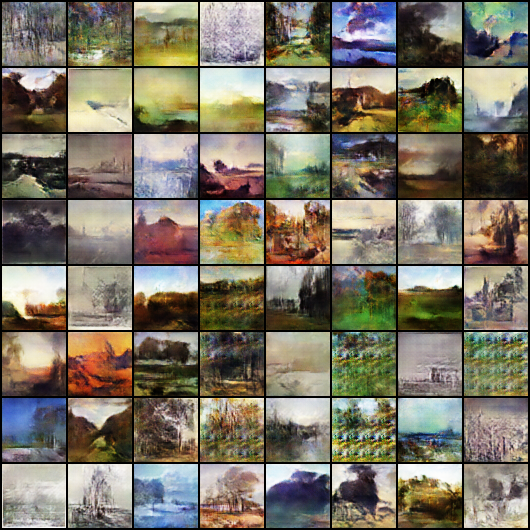
\includegraphics[width=1.0\linewidth]{past_attempts/monet/DCGAN_1/images/epoch328_generator}
					\caption[]{Epoch 328 of model 3}
					\label{fig:cgm:epoch328generator}
				\end{figure}

				By epoch 354, the texture has developed further, possibly even including diagonal divisions.
				Compare figure \ref{fig:cgm:epoch354generator} with figure \ref{fig:cgvg:epoch0943generator}.
				\begin{figure}
					\centering
					\includegraphics[width=1.0\linewidth]{past_attempts/monet/DCGAN_1/images/epoch354_generator}
					\caption[]{Epoch 354 of model 3}
					\label{fig:cgm:epoch354generator}
				\end{figure}

				At epoch 369, some preliminary details are beginning to form.
				Some of the generated images in figure \ref{fig:cgm:epoch369generator} resemble skyscapes, and others resemble landscapes.
				\begin{figure}
					\centering
					\includegraphics[width=1.0\linewidth]{past_attempts/monet/DCGAN_1/images/epoch369_generator}
					\caption[]{Epoch 369 of model 3}
					\label{fig:cgm:epoch369generator}
				\end{figure}

				At epoch 393, the texture is fading, and details are becoming somewhat more clear.
				Figure \ref{fig:cgm:epoch393generator} shows multiple different types of painting developing.
				\begin{figure}
					\centering
					\includegraphics[width=1.0\linewidth]{past_attempts/monet/DCGAN_1/images/epoch393_generator}
					\caption[]{Epoch 393 of model 3}
					\label{fig:cgm:epoch393generator}
				\end{figure}

				At epoch 411, some texture is reappearing.
				More color variation is visible in the images that are primarily green.
				See figure \ref{fig:cgm:epoch411generator}.
				\begin{figure}
					\centering
					\includegraphics[width=1.0\linewidth]{past_attempts/monet/DCGAN_1/images/epoch411_generator}
					\caption[]{Epoch 411 of model 3}
					\label{fig:cgm:epoch411generator}
				\end{figure}

				At epoch 439, the texture is receding again, and some of the seascape-like images are quite good.
				See figure \ref{fig:cgm:epoch439generator}.
				\begin{figure}
					\centering
					\includegraphics[width=1.0\linewidth]{past_attempts/monet/DCGAN_1/images/epoch439_generator}
					\caption[]{Epoch 439 of model 3}
					\label{fig:cgm:epoch439generator}
				\end{figure}

				Epoch 468, shown in figure \ref{fig:cgm:epoch468generator}, has once again formed a texture.
				\begin{figure}
					\centering
					\includegraphics[width=1.0\linewidth]{past_attempts/monet/DCGAN_1/images/epoch468_generator}
					\caption[]{Epoch 468 of model 3}
					\label{fig:cgm:epoch468generator}
				\end{figure}

				The images from epoch 483, shown in figure \ref{fig:cgm:epoch483generator}, have once again become less textured.
				\begin{figure}
					\centering
					\includegraphics[width=1.0\linewidth]{past_attempts/monet/DCGAN_1/images/epoch483_generator}
					\caption[]{Epoch 483 of model 3}
					\label{fig:cgm:epoch483generator}
				\end{figure}

				Epochs 492 and 498 both produce some decent images.
				Although this model was trained through epoch 500, it is likely that one of these two epochs produced the best images.
				Compare figures \ref{fig:cgm:epoch492generator} and \ref{fig:cgm:epoch498generator}.
				This model was somewhat successful.
				It may have continued to improve if we had continued training, but at this point in the project we had moved away from attempting to train a single model for as long as possible.
				\begin{figure}
					\centering
					\includegraphics[width=1.0\linewidth]{past_attempts/monet/DCGAN_1/images/epoch492_generator}
					\caption[]{Epoch 492 of model 3}
					\label{fig:cgm:epoch492generator}
				\end{figure}

				\begin{figure}
					\centering
					\includegraphics[width=1.0\linewidth]{past_attempts/monet/DCGAN_1/images/epoch498_generator}
					\caption[]{Epoch 498 of model 3}
					\label{fig:cgm:epoch498generator}
				\end{figure}

				We also trained a model on the Monet dataset converted to grayscale in the hope that fewer color channels may simplify the calculations and therefore speed up the training, but this hypothesis turned out to be false.

				Figure \ref{fig:cgm:gray:epoch500generator} shows the end result of that model's training.
				As can be seen from the images, virtually no progress was made, despite training for the same number of epochs as model 3.
				\begin{figure}
					\centering
					\includegraphics[width=1.0\linewidth]{past_attempts/monet/DCGAN_2/images/epoch500_generator}
					\caption{Epoch 500 of a model trained on a grayscale version of the Monet dataset.}
					\label{fig:cgm:gray:epoch500generator}
				\end{figure}

				For comparison, figure \ref{fig:cgm:epoch498grayscale} is the image from figure \ref{fig:cgm:epoch498generator}, converted to grayscale.
				This is what we were expecting figure \ref{fig:cgm:gray:epoch500generator} to look like.
				\begin{figure}
					\centering
					\includegraphics[width=1.0\linewidth]{past_attempts/monet/DCGAN_1/epoch498grayscale}
					\caption{Figure \ref{fig:cgm:epoch498generator}, converted to grayscale. This is what we had expected figure \ref{fig:cgm:gray:epoch500generator} to look like.}
					\label{fig:cgm:epoch498grayscale}
				\end{figure}

			\subsubsection{Model 4: WikiArt Images, 64 pixels}
				This model made remarkable progress very quickly.
				It spends a few epochs trying random colors (see figure \ref{fig:wa64:epoch004generator}), but quickly progresses.
				\begin{figure}
					\centering
					\includegraphics[width=1.0\linewidth]{past_attempts/landscapes/64x64/images/epoch004_generator}
					\caption{Epoch 4 of model 4.}
					\label{fig:wa64:epoch004generator}
				\end{figure}

				By epoch 21 (figure \ref{fig:wa64:epoch021generator}), the model seems to have learned that the sky is a lighter color than the ground.
				\begin{figure}
					\centering
					\includegraphics[width=1.0\linewidth]{past_attempts/landscapes/64x64/images/epoch021_generator}
					\caption{Epoch 21 of model 4.}
					\label{fig:wa64:epoch021generator}
				\end{figure}

				By epoch 39 (figure \ref{fig:wa64:epoch039generator}), the sky and ground are very clearly defined, and objects are beginning to form in the midground and background of the image.
				\begin{figure}
					\centering
					\includegraphics[width=1.0\linewidth]{past_attempts/landscapes/64x64/images/epoch039_generator}
					\caption{Epoch 39 of model 4.}
					\label{fig:wa64:epoch039generator}
				\end{figure}

				At epoch 50, many images have static, but details are developing.
				See figure \ref{fig:wa64:epoch050generator}
				\begin{figure}
					\centering
					\includegraphics[width=1.0\linewidth]{past_attempts/landscapes/64x64/images/epoch050_generator}
					\caption{Epoch 50 of model 4.}
					\label{fig:wa64:epoch050generator}
				\end{figure}

				At epoch 76, the static is receding, and details are becoming clearer (figure \ref{fig:wa64:epoch076generator}).
				\begin{figure}
					\centering
					\includegraphics[width=1.0\linewidth]{past_attempts/landscapes/64x64/images/epoch076_generator}
					\caption{Epoch 76 of model 4.}
					\label{fig:wa64:epoch076generator}
				\end{figure}

				At epoch 99, the static has returned, but fine details are continuing to develop.
				See figure \ref{fig:wa64:epoch099generator}.
				\begin{figure}
					\centering
					\includegraphics[width=1.0\linewidth]{past_attempts/landscapes/64x64/images/epoch099_generator}
					\caption{Epoch 99 of model 4.}
					\label{fig:wa64:epoch099generator}
				\end{figure}

				At epoch 125, the static appears to be somewhat smoothing out.
				No image appears to be attempted twice; each generated image is unique.
				See figure \ref{fig:wa64:epoch125generator}.
				\begin{figure}
					\centering
					\includegraphics[width=1.0\linewidth]{past_attempts/landscapes/64x64/images/epoch125_generator}
					\caption{Epoch 125 of model 4.}
					\label{fig:wa64:epoch125generator}
				\end{figure}

				At epoch 150, the static has come back in some images, but others are starting to look convincing.
				The model appears to have learned how to mimic the sky portion of images more quickly than the ground portion.
				See figure \ref{fig:wa64:epoch150generator}.
				\begin{figure}
					\centering
					\includegraphics[width=1.0\linewidth]{past_attempts/landscapes/64x64/images/epoch150_generator}
					\caption{Epoch 150 of model 4.}
					\label{fig:wa64:epoch150generator}
				\end{figure}

				Epoch 175 shows continued development of the images.
				There is very little static, but not enough of the images are detailed enough to be convincing.
				See figure \ref{fig:wa64:epoch175generator}.
				\begin{figure}
					\centering
					\includegraphics[width=1.0\linewidth]{past_attempts/landscapes/64x64/images/epoch175_generator}
					\caption{Epoch 175 of model 4.}
					\label{fig:wa64:epoch175generator}
				\end{figure}

				Epoch 201 has static returning, but otherwise appears to be making progress.
				See figure \ref{fig:wa64:epoch201generator}.
				\begin{figure}
					\centering
					\includegraphics[width=1.0\linewidth]{past_attempts/landscapes/64x64/images/epoch201_generator}
					\caption{Epoch 201 of model 4.}
					\label{fig:wa64:epoch201generator}
				\end{figure}

				In epoch 225's images, the static has still not resolved itself compared to the last checkpoint.
				See figure \ref{fig:wa64:epoch225generator}.
				\begin{figure}
					\centering
					\includegraphics[width=1.0\linewidth]{past_attempts/landscapes/64x64/images/epoch225_generator}
					\caption{Epoch 225 of model 4.}
					\label{fig:wa64:epoch225generator}
				\end{figure}

				The images from epoch 250 have less static than those from epoch 225.
				Additionally, the image in the top row and third from the right in figure \ref{fig:wa64:epoch250generator} appears to us to have developed human figures.
				This surprised us, as we were not aware that this dataset contained anything except for landscapes.
				\begin{figure}
					\centering
					\includegraphics[width=1.0\linewidth]{past_attempts/landscapes/64x64/images/epoch250_generator}
					\caption{Epoch 250 of model 4.}
					\label{fig:wa64:epoch250generator}
				\end{figure}

				At epoch 275, the static has faded further, and some images are becoming very detailed.
				See figure \ref{fig:wa64:epoch275generator}.
				\begin{figure}
					\centering
					\includegraphics[width=1.0\linewidth]{past_attempts/landscapes/64x64/images/epoch275_generator}
					\caption{Epoch 275 of model 4.}
					\label{fig:wa64:epoch275generator}
				\end{figure}

				Epoch 298 has almost no static present, and more of the images are becoming convincing.
				See figure \ref{fig:wa64:epoch298generator}.
				\begin{figure}
					\centering
					\includegraphics[width=1.0\linewidth]{past_attempts/landscapes/64x64/images/epoch298_generator}
					\caption{Epoch 298 of model 4.}
					\label{fig:wa64:epoch298generator}
				\end{figure}

				At epoch 328, only a few images have any static at all, and nearly all of the rest look highly convincing.
				See figure \ref{fig:wa64:epoch328generator}.
				\begin{figure}
					\centering
					\includegraphics[width=1.0\linewidth]{past_attempts/landscapes/64x64/images/epoch328_generator}
					\caption{Epoch 328 of model 4.}
					\label{fig:wa64:epoch328generator}
				\end{figure}

				Epoch 350's images have a similarly high level of detail to those from epoch 328, and the remaining static is starting to smooth out.
				See figure \ref{fig:wa64:epoch350generator}.
				\begin{figure}
					\centering
					\includegraphics[width=1.0\linewidth]{past_attempts/landscapes/64x64/images/epoch350_generator}
					\caption{Epoch 350 of model 4.}
					\label{fig:wa64:epoch350generator}
				\end{figure}

				At epoch 375, virtually all of the images pass as originals.
				There are still some with static, but they are greatly outnumbered.
				See figure \ref{fig:wa64:epoch375generator}.
				\begin{figure}
					\centering
					\includegraphics[width=1.0\linewidth]{past_attempts/landscapes/64x64/images/epoch375_generator}
					\caption{Epoch 375 of model 4.}
					\label{fig:wa64:epoch375generator}
				\end{figure}

				Epoch 400's images do not show a distinct improvement over those from epoch 375.
				It is possible that this model's performance has peaked.

				We consider this model to have been successful.
				This is consistent with the results seen by Jones and Bonafilia\cite{otherGanGogh}.
				\begin{figure}
					\centering
					\includegraphics[width=1.0\linewidth]{past_attempts/landscapes/64x64/images/epoch400_generator}
					\caption{Epoch 400 of model 4.}
					\label{fig:wa64:epoch400generator}
				\end{figure}
			\subsubsection{Model 5: WikiArt Images, 128 pixels}
				At epoch 24, model 5's process is comparable to model 4.
				Compare figures \ref{fig:wa64:epoch021generator} and \ref{fig:wa128:epoch024generator}.
				\begin{figure}
					\centering
					\includegraphics[width=1.0\linewidth]{past_attempts/landscapes/128x128/images/epoch024_generator}
					\caption{Epoch 24 of model 5.}
					\label{fig:wa128:epoch024generator}
				\end{figure}

				Epoch 50's images are also approximately as expected.
				See figure \ref{fig:wa128:epoch050generator}.
				\begin{figure}
					\centering
					\includegraphics[width=1.0\linewidth]{past_attempts/landscapes/128x128/images/epoch050_generator}
					\caption{Epoch 50 of model 5.}
					\label{fig:wa128:epoch050generator}
				\end{figure}

%				\begin{figure}
%					\centering
%					\includegraphics[width=1.0\linewidth]{past_attempts/landscapes/128x128/images/epoch100_generator}
%					\caption{Epoch 100 of model 5.}
%					\label{fig:wa128:epoch100generator}
%				\end{figure}
%
%				\begin{figure}
%					\centering
%					\includegraphics[width=1.0\linewidth]{past_attempts/landscapes/128x128/images/epoch150_generator}
%					\caption{Epoch 150 of model 5.}
%					\label{fig:wa128:epoch150generator}
%				\end{figure}

				This continues generally as expected for a while.
				However, by epoch 200, it becomes extremely clear that image diversity has plummeted.
				Most of the images in figure \ref{fig:wa128:epoch200generator} are slight variations on the same four or so base images.
				We are not sure what caused this to happen so early in the training.
				Models 1 and 2 did not exhibit this behavior until making significantly more progress.
				\begin{figure}
					\centering
					\includegraphics[width=1.0\linewidth]{past_attempts/landscapes/128x128/images/epoch200_generator}
					\caption{Epoch 200 of model 5.}
					\label{fig:wa128:epoch200generator}
				\end{figure}

				Epoch 250 has less static than epoch 200.
				See figure \ref{fig:wa128:epoch250generator}.
				\begin{figure}
					\centering
					\includegraphics[width=1.0\linewidth]{past_attempts/landscapes/128x128/images/epoch250_generator}
					\caption{Epoch 250 of model 5.}
					\label{fig:wa128:epoch250generator}
				\end{figure}

				At epoch 300, vertical streaks have formed in most of the images.
				This is a different kind of distortion than has been seen elsewhere.
				See figure \ref{fig:wa128:epoch300generator}.
				\begin{figure}
					\centering
					\includegraphics[width=1.0\linewidth]{past_attempts/landscapes/128x128/images/epoch300_generator}
					\caption{Epoch 300 of model 5.}
					\label{fig:wa128:epoch300generator}
				\end{figure}

				By epoch 350, the streaks are gone, and many of the images are getting clearer, although image diversity is still low.
				See figure \ref{fig:wa128:epoch350generator}.
				\begin{figure}
					\centering
					\includegraphics[width=1.0\linewidth]{past_attempts/landscapes/128x128/images/epoch350_generator}
					\caption{Epoch 350 of model 5.}
					\label{fig:wa128:epoch350generator}
				\end{figure}

				At epoch 400, there is very little static, but several of the images have developed a textured appearance.
				See figure \ref{fig:wa128:epoch400generator}.
				\begin{figure}
					\centering
					\includegraphics[width=1.0\linewidth]{past_attempts/landscapes/128x128/images/epoch400_generator}
					\caption{Epoch 400 of model 5.}
					\label{fig:wa128:epoch400generator}
				\end{figure}

				Epoch 450's images are mostly as expected, however two of the images are surrounded by a white border.
				We are not sure where this feature came from.
				See figure \ref{fig:wa128:epoch450generator}.
				\begin{figure}
					\centering
					\includegraphics[width=1.0\linewidth]{past_attempts/landscapes/128x128/images/epoch450_generator}
					\caption{Epoch 450 of model 5.}
					\label{fig:wa128:epoch450generator}
				\end{figure}

				The images from epoch 500 are mostly decent quality, aside from the low variation.
				See figure \ref{fig:wa128:epoch500generator}.
				\begin{figure}
					\centering
					\includegraphics[width=1.0\linewidth]{past_attempts/landscapes/128x128/images/epoch500_generator}
					\caption{Epoch 500 of model 5.}
					\label{fig:wa128:epoch500generator}
				\end{figure}

				However, by epoch 550, many of the images appear to have collapsed into static.
				Additionally, image diversity is even lower than it had been, with most of the images being a variation of only two base images.
				See figure \ref{fig:wa128:epoch550generator}.
				\begin{figure}
					\centering
					\includegraphics[width=1.0\linewidth]{past_attempts/landscapes/128x128/images/epoch550_generator}
					\caption{Epoch 550 of model 5.}
					\label{fig:wa128:epoch550generator}
				\end{figure}

				By epoch 600, image diversity has improved marginally.
				Many images are still static.
				See figure \ref{fig:wa128:epoch600generator}.
				\begin{figure}
					\centering
					\includegraphics[width=1.0\linewidth]{past_attempts/landscapes/128x128/images/epoch600_generator}
					\caption{Epoch 600 of model 5.}
					\label{fig:wa128:epoch600generator}
				\end{figure}

				At epoch 650, some of the images are decent again.
				Only a few images have static, although image diversity is still terrible.
				See figure \ref{fig:wa128:epoch650generator}.
				\begin{figure}
					\centering
					\includegraphics[width=1.0\linewidth]{past_attempts/landscapes/128x128/images/epoch650_generator}
					\caption{Epoch 650 of model 5.}
					\label{fig:wa128:epoch650generator}
				\end{figure}

				At epoch 700, a couple of images are somewhat convincing.
				See figure \ref{fig:wa128:epoch700generator}.

				This model did not behave that way that we had expected it to.
				Many questions remain about why it was so much less successful than model 4.
				\begin{figure}
					\centering
					\includegraphics[width=1.0\linewidth]{past_attempts/landscapes/128x128/images/epoch700_generator}
					\caption{Epoch 700 of model 5.}
					\label{fig:wa128:epoch700generator}
				\end{figure}

	\section{Conclusion}
		Our research has emphasized a key detail in machine learning: you need a very large dataset to get good results.
		This was shown by our models failing to converge with smaller dataset sizes.
		The datasets with 211, 400, and even 1,000 images all failed to converge.
		% failed to converge upone what
		% because they had converged to certain choices, such as color selection/ pallete
		% or horizonal deliniation (eg there's a surface (land/sea) and a sky) for the relevant data set


		The model with the smallest dataset that achieved convincing results was trained on 15,000 images.
		Future research may include determining the threshold more precisely, as there is still a large gap between 1,000 and 15,000.
		Due to this inherent limiting requirement, it seems that our initial goal of computationally determining what characteristics define Van Gogh's art was likely unattainable.

\appendix
	\section{Appendix: Weekly Progress}
		\subsection{Weeks 1-3}
		\label{subsec:weekly:1-3}
			\subsubsection{Work Completed}
				During this time period, we tested sample code from the TorchGAN\cite{pal2019torchgan} project using data from the MNIST\cite{lecun2010mnist} dataset.
				We also began writing code to provide an interface for the TorchGAN code to read from the training data we had previously collected from the Van Gogh Museum (e.g., \cite{001}, \cite{002}, \cite{003}).
			\subsubsection{Importance of Work}
				Training on the MNIST dataset demonstrated the validity of the training code.
				By verifying the results in this way, we can state with confidence that any deviation is due to the dataset, rather than the code.
			\subsubsection{Problems Encountered}
				After working on writing a subclass to use as an interface between the code and the image data, we discovered that the code was redundant, as there was a general-purpose class included in TorchGAN that could be used for that exact purpose.
				This was a setback, but ultimately allowed us to continue to move forward without having to worry about testing custom code.

		\subsection{Weeks 4-6}
			\subsubsection{Work Completed}
				This period of the project was almost entirely spent on training the model on the Van Gogh Museum dataset.
				We decided that, for the sake of reliability and availability, we would train the model locally.
			\subsubsection{Importance of Work}
				Training the model represents the bulk of the work of this project.
				While a certain amount of time has to be allocated for setting things up, the real results of the project are the models produced by training, as well as the images generated by those models.
			\subsubsection{Problems Encountered}
				Due to the hardware configuration available locally, we were not able to utilize GPU acceleration for our training.
				This meant slower training, but should not affect the quality of results, as the MNIST test was successful under the same conditions.
				Additionally, despite running the model for 8000 epochs of training, we did not achieve the expected results, and were concerned about potential overfitting.

		\subsection{Weeks 7-8}
			\subsubsection{Work Completed}
				After our first attempt did not yield results, we began looking into alternate approaches.
				While researching other GAN types that could be used, we discovered that the researchers from the CycleGAN\cite{CycleGAN2017}\cite{isola2017image} project had compiled their own Van Gogh dataset.
				The CycleGAN Van Gogh dataset consisted of 400 pictures from WikiArt\cite{wikiartVanGogh}, which was nearly twice as many images as the 211 we had been able to gather from the Van Gogh Museum.
				Additionally, the CycleGAN researchers had compiled a similar dataset of 1072 paintings by Claude Monet, also from WikiArt.
				We then began training a new model on the CycleGAN Van Gogh dataset.
			\subsubsection{Importance of Work}
				Since we knew from previous research that performance of neural networks generally improves with larger training data, these new datasets represented an unexpected opportunity to improve the quality of our results.
			\subsubsection{Problems Encountered}
				Unfortunately, even with this larger dataset, the GAN did not produce clear images.
				The color palettes of the generated images were reminiscent of a Van Gogh painting, but no clearly defined features were present.
				Any apparent features were extremely vague, and concerns about the Rorschach effect were raised.

				Additionally, since the CycleGAN dataset was nearly twice as big as the Van Gogh Museum dataset, training times increased proportionally.
				This meant that fewer epochs of training were able to be completed in the same amount of time.

		\subsection{Week 9}
			\subsubsection{Work Completed}
				At this point, we decided to try a somewhat different tactic.
				We decided to switch to the Monet dataset, and test different ways of approaching the task in order to try to figure out which might work best.
				Variables to be tested include the specific GAN being used, including both supervised and unsupervised GANs, and whether color or grayscale images would be used.
			\subsubsection{Importance of Work}
				This approach allows us to test a number of possible methods without fully committing to any of them, instead of spending all of our resources on a single variation and hoping for it to work.
				Additionally, we discovered that another, similar project had been attempted in the past\cite{otherGanGogh}, and that those researchers had encountered the same performance issues as us.
				This lends further credibility to our belief that the size of the Van Gogh datasets was simply too small for the GAN to learn from.
			\subsubsection{Problems Encountered}
				As previously noted, increasing the size of the dataset increases the time required to train the model.
				The Van Gogh Museum dataset took about 35 seconds per epoch, and the CycleGAN Van Gogh dataset took about 70.
				However, the Monet dataset takes nearly two and a half minutes per epoch, which severely limits the number of epochs that can be completed.

		\subsection{Week 10}
			\subsubsection{Work Completed}
				After speaking with our advisor this week, we decided to change focus once again.
				Our current goal is to attempt to replicate the results of the other GANGogh project \cite{otherGanGogh}.
				We are training a model on the dataset of landscape paintings that Jones and Bonafilia compiled from WikiArt.
				This has so far been much more successful than previous attempts with other datasets.
			\subsubsection{Importance of Work}
				If we are able to reproduce the results of Jones and Bonafilia, it will further confirm that the problems we encountered with the Van Gogh datasets was due to their size.
			\subsubsection{Problems Encountered}
				At 15,000 images, the landscapes dataset is much larger than any of our previous datasets, with the sole exception of the MNIST dataset.
				Despite reducing the size of the training images to 64 by 64 pixels, this dataset still takes between 5 and 15 minutes\footnote{Most epochs take 5 minutes, but occasionally one will take two or three times that long, presumably due to other applications running at the same time. This is, however, a much greater variance than has been observed with other datasets, even under the same conditions.} per epoch of training.
				However, unlike previous time-consuming training attempts, this one appears to be making significant progress.
				The small size of the images limits the amount of detail that can be shown, but after 400 epochs, the model is consistently producing convincing images.

		\subsection{Weeks 11-13}
			\subsubsection{Work Completed}
				After successfully reproducing the results of Jones and Bonafilia at a resolution of 64 by 64 pixels, we attempted the same task, but at a resolution of 128 by 128 pixels.

			\subsubsection{Importance of Work}
				While the 64 by 64 images were convincingly similar to the original images resized to that resolution, the small size limits the amount of detail able to be shown.
				The ability to generate similarly convincing, larger images confirms that the GAN is actually learning the patterns that we want it to be learning.

			\subsubsection{Problems Encountered}
				As expected, increasing the resolution increased the length of each epoch of training.
				At 128 by 128 pixels, each epoch takes 10 to 20 minutes.
				Additionally, despite our success with the smaller resolution at 400 epochs, the same number of epochs have not produced the same level of results with this model.
				At 700 epochs, the model is able to produce some convincing images, but not nearly as consistently as the previous model.


\bibliographystyle{IEEEtran}
\bibliography{van_gogh_bib}
\nocite{*}
\end{document}
